% Options for packages loaded elsewhere
\PassOptionsToPackage{unicode}{hyperref}
\PassOptionsToPackage{hyphens}{url}
%
\documentclass[
  10pt,
  ignorenonframetext,
  aspectratio=169,
]{beamer}
\usepackage{pgfpages}
\setbeamertemplate{caption}[numbered]
\setbeamertemplate{caption label separator}{: }
\setbeamercolor{caption name}{fg=normal text.fg}
\beamertemplatenavigationsymbolsempty
% Prevent slide breaks in the middle of a paragraph
\widowpenalties 1 10000
\raggedbottom
\usepackage{amsmath,amssymb}
\usepackage{iftex}
\ifPDFTeX
  \usepackage[T1]{fontenc}
  \usepackage[utf8]{inputenc}
  \usepackage{textcomp} % provide euro and other symbols
\else % if luatex or xetex
  \usepackage{unicode-math} % this also loads fontspec
  \defaultfontfeatures{Scale=MatchLowercase}
  \defaultfontfeatures[\rmfamily]{Ligatures=TeX,Scale=1}
\fi
\usepackage{lmodern}
\usetheme[]{Frankfurt}
\ifPDFTeX\else
  % xetex/luatex font selection
\fi
% Use upquote if available, for straight quotes in verbatim environments
\IfFileExists{upquote.sty}{\usepackage{upquote}}{}
\IfFileExists{microtype.sty}{% use microtype if available
  \usepackage[]{microtype}
  \UseMicrotypeSet[protrusion]{basicmath} % disable protrusion for tt fonts
}{}
\makeatletter
\@ifundefined{KOMAClassName}{% if non-KOMA class
  \IfFileExists{parskip.sty}{%
    \usepackage{parskip}
  }{% else
    \setlength{\parindent}{0pt}
    \setlength{\parskip}{6pt plus 2pt minus 1pt}}
}{% if KOMA class
  \KOMAoptions{parskip=half}}
\makeatother
\usepackage{xcolor}
\newif\ifbibliography
\usepackage{graphicx}
\makeatletter
\def\maxwidth{\ifdim\Gin@nat@width>\linewidth\linewidth\else\Gin@nat@width\fi}
\def\maxheight{\ifdim\Gin@nat@height>\textheight\textheight\else\Gin@nat@height\fi}
\makeatother
% Scale images if necessary, so that they will not overflow the page
% margins by default, and it is still possible to overwrite the defaults
% using explicit options in \includegraphics[width, height, ...]{}
\setkeys{Gin}{width=\maxwidth,height=\maxheight,keepaspectratio}
% Set default figure placement to htbp
\makeatletter
\def\fps@figure{htbp}
\makeatother
\ifLuaTeX
  \usepackage{luacolor}
  \usepackage[soul]{lua-ul}
\else
  \usepackage{soul}
  \makeatletter
  \let\HL\hl
  \renewcommand\hl{% fix for beamer highlighting
    \let\set@color\beamerorig@set@color
    \let\reset@color\beamerorig@reset@color
    \HL}
  \makeatother
\fi
\setlength{\emergencystretch}{3em} % prevent overfull lines
\providecommand{\tightlist}{%
  \setlength{\itemsep}{0pt}\setlength{\parskip}{0pt}}
\setcounter{secnumdepth}{-\maxdimen} % remove section numbering
\ifLuaTeX
\usepackage[bidi=basic]{babel}
\else
\usepackage[bidi=default]{babel}
\fi
\babelprovide[main,import]{spanish}
% get rid of language-specific shorthands (see #6817):
\let\LanguageShortHands\languageshorthands
\def\languageshorthands#1{}
\usepackage{graphicx}
\usepackage{mhchem}
\titlegraphic{
\includegraphics[width=2.25cm]{./images/unmsm2.png}}
\logo{
\includegraphics[width=1cm]{./images/unmsm.png}}
\ifLuaTeX
  \usepackage{selnolig}  % disable illegal ligatures
\fi
\usepackage{bookmark}
\IfFileExists{xurl.sty}{\usepackage{xurl}}{} % add URL line breaks if available
\urlstyle{same}
\hypersetup{
  pdftitle={Reacciones Químicas},
  pdfauthor={Grupo 5},
  pdflang={es-PE},
  hidelinks,
  pdfcreator={LaTeX via pandoc}}

\title{Reacciones Químicas}
\subtitle{Ecuaciones diferenciales ordinarias}
\author{Grupo 5}
\date{\today{}}
\institute{Universidad Nacional Mayor de San Marcos}

\begin{document}
\frame{\titlepage}

\begin{frame}[allowframebreaks]
  \tableofcontents[hideallsubsections]
\end{frame}
\begin{frame}{Integrantes}
\phantomsection\label{integrantes}
\begin{enumerate}
\tightlist
\item
  Espinoza Huaman, Diego Alexhander
\item
  Tanaka Matheus, Louiggi
\item
  Linares Rojas, Ander Rafael
\item
  Vilchez Quispe, Yoshiro Cardich
\item
  Solimano Cure, Franco David
\item
  Porras Anco, Sebastian Aaron
\item
  Madrid Llanos, Karla Patricia
\end{enumerate}
\end{frame}

\section{Marco Teórico}\label{marco-teuxf3rico}

\begin{frame}{Marco Teórico}
\begin{columns}[T]
\begin{column}{0.7\textwidth}
\begin{itemize}
\tightlist
\item
  La \ul{\textbf{cinética química}} estudia la velocidad a la cual
  ocurren las reacciones químicas y los factores que influyen en esta
  velocidad.
\item
  Las \ul{\textbf{reacciones químicas}} es un proceso en el cual una o
  más sustancias, denominadas reactivos, se transforman en una o más
  sustancias diferentes, denominadas productos
\item
  Dos tipos de reacciones:

  \begin{itemize}
  \tightlist
  \item
    \textbf{Reacciones de Primer Orden:} la velocidad que depende
    linealmente de la concentración de un reactivo.

    \begin{itemize}
    \tightlist
    \item
      \(X(t)\) es la concentración de la sustancia \(A\) en el tiempo
      \(t\).
    \item
      \(k\) es la constante de velocidad de reacción (con \(k>0\)).
    \end{itemize}
  \item
    \textbf{Reacciones de Segundo Orden:} la velocidad de reacción
    depende del producto de las concentraciones de dos reactivos.

    \begin{itemize}
    \tightlist
    \item
      \(\alpha, \beta\): cantidades de los químicos \(A\) y \(B\)
      \((t=0)\)
    \item
      \(X(t)\): la cantidad de sustancia en el tiempo \(t\).
    \item
      \(k\): constante de proporcionalidad
    \end{itemize}
  \end{itemize}
\end{itemize}
\end{column}

\begin{column}{0.3\textwidth}
\(~\)

\(~\)

\[\frac{dX}{dt} = -kX\]

\(~\)

\[\ce{A + B -> C}\]

\[\frac{dX}{dt} = k(\alpha - X)(\beta - X)\]
\end{column}
\end{columns}
\end{frame}

\begin{frame}
\begin{itemize}
\item
  \ul{\textbf{Aplicaciones}}

  \begin{itemize}
  \tightlist
  \item
    \textbf{Decaimiento radiactivo:} La desintegración de isótopos
    radiactivos sigue una cinética de primer orden.
  \item
    \textbf{Reacciones enzimáticas:} Algunas reacciones catalizadas por
    enzimas pueden aproximarse por cinéticas de segundo orden.
  \item
    \textbf{Farmacocinética:} La absorción y eliminación de fármacos del
    cuerpo a menudo se modelan utilizando cinéticas de primer o segundo
    orden, dependiendo de la naturaleza del proceso.
  \end{itemize}
\end{itemize}

\(~\)

\begin{columns}[T]
\begin{column}{0.48\textwidth}
\begin{figure}
\centering
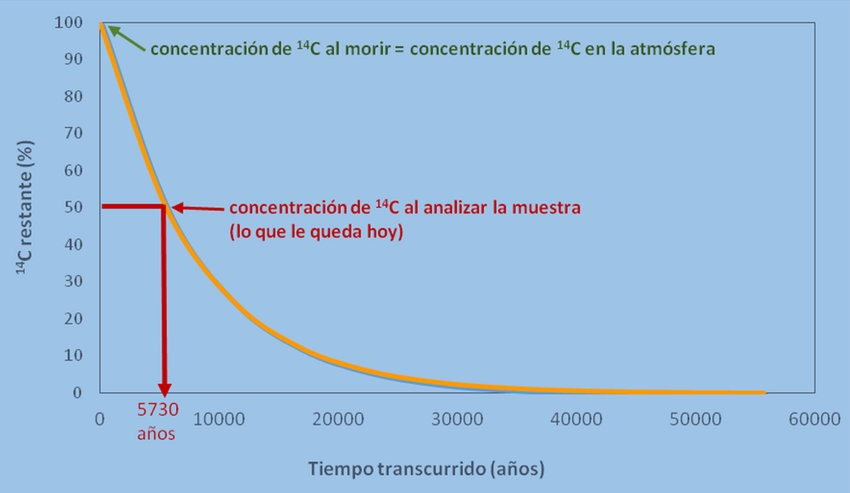
\includegraphics[width=\textwidth,height=0.35\textheight]{./images/grafico.jpg}
\caption{Decaimiento}
\end{figure}
\end{column}

\begin{column}{0.48\textwidth}
\begin{figure}
\centering
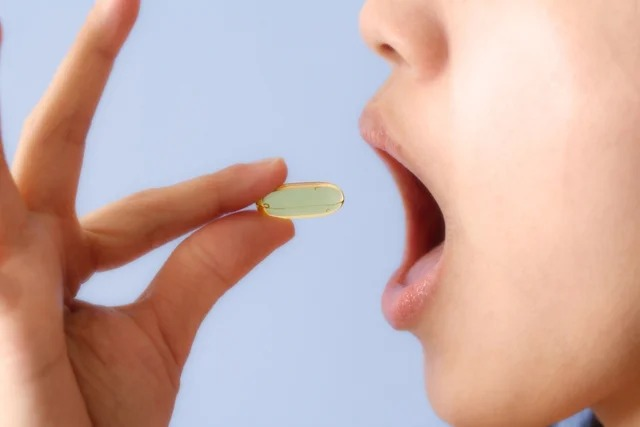
\includegraphics[width=\textwidth,height=0.35\textheight]{./images/pastilla.jpg}
\caption{Farmacocinética}
\end{figure}
\end{column}
\end{columns}
\end{frame}

\section{Ejemplos}\label{ejemplos}

\begin{frame}{Ejemplo 1}
\phantomsection\label{ejemplo-1}
\begin{block}{Enunciado}
\phantomsection\label{enunciado}
Un compuesto \(C\) se forma cuando se combinan dos sustancias químicas
\(A\) y \(B\). La relación resultante entre las dos sustancias químicas
es tal que por cada gramo de \(A\) se utilizan \(4 g\) de \(B\). Se
observa que se forman \(30 g\) del compuesto \(C\) en 10 minutos.
Determine la cantidad de \(C\) en el tiempo \(t\) si la velocidad de la
reacción es proporcional a las cantidades restantes de \(A\) y \(B\), si
inicialmente hay \(50 g\) de \(A\) y \(32 g\) de \(B\). ¿Qué cantidad
del compuesto \(C\) hay a los 15 minutos
\end{block}

\begin{block}{Desarrollo}
\phantomsection\label{desarrollo}
\begin{columns}[T]
\begin{column}{0.48\textwidth}
\[\begin{split}
\ce{A + B & -> C} \\
A + B = C & \text{, pero} \quad 4A = B \\
A = \frac{C}{5} & \rightarrow{} B = \frac{4C}{5} \\
\frac{dC}{dt} = k(50 - & A)(32 - B) \\
\end{split}\]
\end{column}

\begin{column}{0.48\textwidth}
\[\begin{split}
\frac{dC}{dt} & = k\left(50 - \frac{C}{5}\right) \left(32 - \frac{4C}{5}\right) \\
\frac{dC}{dt} & = k(250 - C)(40 - C) \\
\end{split}\]
\end{column}
\end{columns}
\end{block}
\end{frame}

\begin{frame}{Ejemplo 5}
\phantomsection\label{ejemplo-5}
\begin{block}{Enunciado}
\phantomsection\label{enunciado-1}
En la reacción de tercer orden o trimolecular
\(\ce{A + B + C -> M + N}\), \(a\), \(b\) y \(c\) moles por litro de
\(A\), \(B\) y \(C\) se combinan. Si \(x\) denota el número de moles por
litro de \(A\), \(B\) o \(C\) que han reaccionado después de un tiempo
\(t\) (0 el número de moles por litro de \(M\) o \(N\) que se han
formado), entonces la tasa de la reacción está dada por:

\[\dfrac{dx}{dt}=k(a-x)(b-x)(c-x)\]

Si a, b y c son diferentes y x(0)=0, resolver la EDO
\end{block}
\end{frame}

\begin{frame}
\begin{block}{Desarrollo}
\phantomsection\label{desarrollo-1}
\[\begin{split}
\dfrac{dx}{(a-x)(b-x)(c-x)} = k dt \\
\end{split}\]
\end{block}
\end{frame}

\section{Gracias por su atención}\label{gracias-por-su-atenciuxf3n}

\begin{frame}{Gracias por su atención}
\begin{center}


\includegraphics[width=0.6\textwidth,height=\textheight]{./images/dog.png}

\end{center}
\end{frame}

\end{document}
